\section{Pasaaltos, Pasabandas y Rechazabandas}

Es importante mencionar antes de iniciar el análisis que puesto a que los tres filtros tienen los mismo componentes y viendo las ecuaciones deducidas en el anexo (de las cuales se hablará más adelante), todos los circuitos poseen la misma frecuencia de corte. 
\begin{figure}[h!]
    \centering

    \begin{minipage}[b]{0.32\textwidth}
        \centering
        \resizebox{\linewidth}{!}{
        \begin{tikzpicture}[transform shape]
	\draw (-11, 4) to[american voltage source] (-11, 2);
	\node[buffer, xscale=0.66, yscale=0.66] at (-10.038, 4){};
	\draw (-11, 4) -- (-10.5, 4);
	\draw (-9.576, 4) to[american resistor, l={$R$}] (-7.988, 4);
	\draw (-7.988, 4) to[capacitor, l={$C$}] (-6.5, 4);
	\draw (-6.5, 4) to[american inductor, l={$L$}] (-6.5, 2);
	\draw (-11, 2) -- (-6.5, 2);
	\node at (-6.375, 4.125){$v_{out}$};
	\node at (-11, 4.125){$v_{in}$};
        \end{tikzpicture}}
        \caption{Pasaaltos}
        \label{fig:pasaaltos}
    \end{minipage}
    \hfill
    \begin{minipage}[b]{0.32\textwidth}
        \centering
        \resizebox{\linewidth}{!}{
        \begin{tikzpicture}[transform shape]
	\draw (-11, 4) to[american voltage source] (-11, 2);
	\node[buffer, xscale=0.66, yscale=0.66] at (-10.038, 4){};
	\draw (-11, 4) -- (-10.5, 4);
	\draw (-6.5, 4) to[american resistor, l={$R$}] (-6.5, 2);
	\draw (-7.988, 4) to[capacitor, l={$C$}] (-6.5, 4);
	\draw (-9.576, 4) to[american inductor, l={$L$}] (-8, 4);
	\draw (-11, 2) -- (-6.5, 2);
	\node at (-6.375, 4.125){$v_{out}$};
	\node at (-11, 4.125){$v_{in}$};
        \end{tikzpicture}}
        \caption{Pasabandas}
        \label{fig:pasabandas}
    \end{minipage}
    \hfill
    \begin{minipage}[b]{0.32\textwidth}
        \centering
        \resizebox{\linewidth}{!}{
        \begin{tikzpicture}[transform shape]
	\draw (-11, 4) to[american voltage source] (-11, 2);
	\node[buffer, xscale=0.66, yscale=0.66] at (-10.038, 4){};
	\draw (-11, 4) -- (-10.5, 4);
	\draw (-9.576, 4) to[american resistor, l={$R$}] (-6.5, 4);
	\draw (-6.5, 2.75) to[capacitor, l={$C$}] (-6.5, 2);
	\draw (-6.5, 4) to[american inductor, l={$L$}] (-6.5, 2.75);
	\draw (-11, 2) -- (-6.5, 2);
	\node at (-6.375, 4.125){$v_{out}$};
	\node at (-11, 4.125){$v_{in}$};
        \end{tikzpicture}}
        \caption{Notch}
        \label{fig:notch}
    \end{minipage}

\end{figure}
Primero analizaremos la respuesta de cada filtro en función del tiempo. 

\begin{figure}[H]
    \centering

    \begin{minipage}[b]{0.32\textwidth}
        \centering
        \includegraphics[page=2, width=\linewidth]{Graficos.pdf}
        \caption{Pasaaltos}
        \label{fig:pasaaltostiempo}
    \end{minipage}
    \hfill
    \begin{minipage}[b]{0.32\textwidth}
        \centering
        \includegraphics[page=3, width=\linewidth]{Graficos.pdf}
        \caption{Pasabandas}
        \label{fig:pasabandastiempo}
    \end{minipage}
    \hfill
    \begin{minipage}[b]{0.32\textwidth}
        \centering
        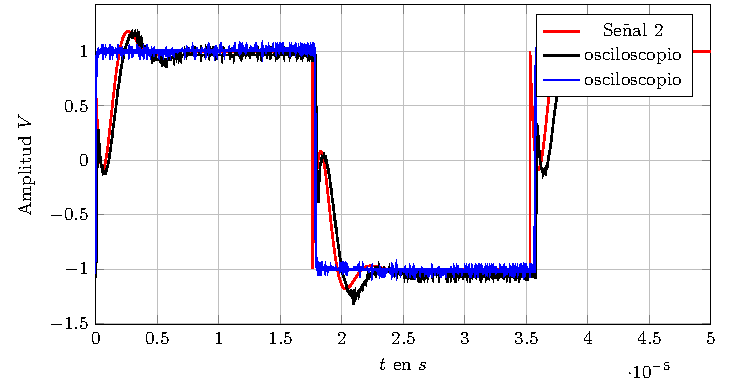
\includegraphics[page=1, width=\linewidth]{Graficos.pdf}
        \caption{Notch}
        \label{fig:notchtiempo}
    \end{minipage}

\end{figure}
Al observar la gráfica de todas las señales, se puede observar que hay una gran correlación en la gráfica obtenida mediante el osciloscopio y la simulada en el ltspice. Una de las principales diferencias que se pueden observar en las tres señales es el desfase en el tiempo. La explicación de esto se debe a la existencia de un buffer a la entrada del circuito el cual añade un efecto de slew-rate. Esto es que el buffer limita la maxima pendiente de subida que la señal puede tener, limitando la velocidad de carga del circuito. Esto termina desenbocando en un desfase en el tiempo del circuito que se puede observar en las tres graficas \ref{fig:pasaaltostiempo}, \ref{fig:pasabandastiempo} y \ref{fig:notchtiempo}
